\chapter{Forward Pass Retracing }
\chaptermark{Forward Pass Retracing: CTC}
\label{chapter:REVEAL}
\newcommand{\cnet}[1][k]{\text{$c$-}\net[#1]}
\newcommand{\lo}[1][j]{l_{#1}}
\newcommand{\clo}[1][j]{\text{$c$-}\lo[#1]}
\newcommand{\djo}[1][j]{d_{#1}}
\newcommand{\NN}{\mathcal{N}}
\newcommand{\HM}{\mathcal{H}}
\newcommand{\cdjo}[1][j]{\text{$c$-}\djo[#1]}
\newcommand{\passto}{\hookrightarrow}
\section{Introduction}


The previous chapter delved into the intricacies of relevance distribution tracing as a technique for assigning significance to complex input features in neural networks. Despite its effectiveness, this approach concluded with an acknowledgment of the challenges posed by high-dimensional Jacobians, particularly their substantial computational and memory requirements. Forward pass retracing is designed to address these limitations, offering a more feasible and efficient method for network interpretation.

At its core, forward pass retracing simplifies the process of determining the contribution of each input feature to the network's output. Unlike the methods discussed in Chapter~\ref{chapter:revLRP}, which involve complex backward propagation techniques and the handling of large Jacobian matrices, forward pass retracing operates by conducting a singular forward pass of the feature through the network. This pass is carried out with modified functions that replicate the network's behaviour during the inference step. By doing so, it directly analyses how the input features influence the output in a more straightforward and computationally less demanding way.

This chapter will comprehensively explore the mechanisms and advantages of forward pass retracing. We will discuss how this method mirrors the network's inference behaviour in a single forward pass. This is achieved without compromising the depth and fidelity of the interpretative insights gleaned from the network. Furthermore, we will delve into the practical implementation of forward pass retracing, highlighting its application across various types of neural network architectures and datasets. Through comprehensive evaluation, we will demonstrate empirically the versatility and effectiveness of this method in providing clear, interpretable insights into how important the neural networks find complex input features. 


\section{Motivation}

Forward pass retracing is a new type of explanation of CNN classifications. This method emphasises the role of complex features in contributing to the final classification, a concept termed as Contribution To Classification (CTC).

\begin{definition}[Contribution]
For a given input vector $\vec{x}\in \bbR^d$ and a given feature $F\subseteq \bbR^2$, we define the \emph{contribution} at layer $k\in \Lambda$ inductively, by taking:
\begin{equation*}
       \vec{c}_k = \Lambda_i^\prime\big(\vec{a}_k,[\vec{a}_j]_{j\passto k},[\vec{c}_j]_{j\passto k}\big)
\end{equation*}
where $\Lambda_i^\prime$ denotes the function that mimics the behaviour of the network at layer $\Lambda_i$, depending on the type of layer $k=0,\dots, N$. The value of the contribution $\vec{c}_k$ depends on the contributions from all preceding layers, as well as activation $\vec{a}_k$ computed during the forward pass.
\end{definition}

This chapter outlines a set of rules for propagating activation from specific input regions through the hidden layers of the network, culminating in a singular CTC value. The computation of a feature's CTC value is facilitated by introducing the Contribution To a Neuron (CTN) value. This value represents the activation a neuron receives as a result of the feature during the forward pass, with the CTC value of a feature being equivalent to the CTN value of the classification output neuron. This propagation of activation, which accounts for the feature's contribution during the forward pass, is distinct from a mere classification of the feature. This distinction is crucial due to the non-linear layers like MaxPooling, which could otherwise pool the contribution of neurons not selected during the forward pass, compromising the explanation's faithfulness.


There is an important differentiation between the CTC value of a feature and its relevance.

While current interpretability methods focus on the importance of a feature as part of the entire input considering the specific classification output (\ie feature relevance), the approach described in this chapter isolates the importance of the feature alone during the forward pass (\ie feature's CTC). Figure~\ref{fig:contribution} illustrates the distinction between a feature's relevance and its CTC value using a specific input (i). When considering each pixel as a distinct feature, techniques like LRP assign significant importance values within the context of the entire input. However, for an individual pixel, the CTC value is generally minimal, as no single pixel notably impacts the overall classification. In contrast, when assessing an amalgamation of simple features (pixels), or a complex feature, the CTC value effectively demonstrates the contribution of the entire region to the classification through a heatmap. To enhance interpretability, complex features are presented in varying colours.


% \begin{figure}[h]
% \centering
% \includegraphics[width=\linewidth]{Sections/img/guitar_dog.pdf}
% 	\caption{ \LRP\ identifies most of the edges in the image as relevant when explaining the ``Electric Guitar'' class including the head of the dog. In contrast, \REVEAL\ attributes only 0.73\% relevance to the head of the dog and 53\% relevance to the actual guitar.}
% 	\label{fig:guitar_dog}
% \end{figure}

The chapter posits that the CTC value provides a more faithful explanation of a feature's importance to the classification than its relevance. In convolutional neural networks, while edges detected from the input are relevant for decision-making, their contribution to the classification can vary significantly. Relevance-based approaches may overestimate the importance of certain input parts, as they may not actively contribute much to the classification. This is particularly evident in deep convolutional neural networks with extensive convolutional layers, where almost all edges are likely to be deemed important. Figure~\ref{fig:guitar_dog} contrasts relevance-propagation methods with this approach, highlighting the difference in the importance assigned to various input parts.


\section{Propagation Rules}

This section defines a set of rules which allow for the contribution to be distributed layer by layer starting from the input layer and finishing with the output layer. These rules differ from just preforming a forward-pass on a complex input feature, as they compute the activation that is a direct result of the presence of the complex input feature during the forward pass, as opposed to computing the activations that this complex input feature has by itself. Given the presence of different layer types, different contribution propagation rules must be defined which respect and reflect the underlying structure of the network and functions that comprise it.

The first rule is the input layer's, where the relevance of each input feature is defined as being the activation of that feature. The concept of "masking" is then introduced, with its role in ensuring that only contributions from active neurons during the inference step are allowed to propagate through the network. The rules that follow describe how the forward pass can be mirrored. All rules try to preserve the signal of the relevance being propagated. This is particularly important when dealing with learned network parameters that may suppress the complex input feature's relevance signal. An example of this can be seen for the bias term added to activations post dense layers and convolutional layers or with batch normalisation layers, which may completely drown the relevance signal post re-scaling. 


\subsection{Contribution of First Layer}

Let the $\NN=\big(\Lambda,\passto,(f_k)_{k\in \Lambda}\big)$ be a trained neural network with a set of layers $\Lambda=\{0,\dots, N\}$, with a single source $0\in \Lambda$, referred to as the input layer and single sink $N\in \Lambda$, referred to as the \emph{output layer}. Each $f_k:\bbR^{n_j}\to \bbR^{m_k}$ describes a vector transformation associated with each layer, with the dimensionality conditions that $m_k=\sum_{j\passto k} n_j$, for all $k=1,\dots N$.


The contribution of a region at the input layer 0 $\in \Lambda$ is the same as the activation's of that region (i.e the pixel values of the three input channels), so the contribution $\vec{c}_0$ is defined as:
\begin{equation*}
    \vec{c}_0 = \vec{a}_0 \odot \vec{m},
\end{equation*}
where $\vec{m}\in \{0,1\}^{n_0}$ is a mask over the region propagated as found by the method describer in Section~\ref{chap:clustering}, and $\odot$ denotes element-wise multiplication operation. Performing the multiplication with the mask sets to zero all the activations of neurons that are not in the region of the feature that is being propagated.

\subsection{Masking After Each Layer}
Only neurons that where active during the inference step should have contributions distributed to them during the feature contribution propagation. Thereby after each layer's function is performed a mask $\vec{m}_k\in \{0,1\}^{n_0}$ is defined over the activations values in $\vec{a}_k$, as follows 
\begin{equation*}
    \label{eq:masking}
    m_k(i) = \begin{cases}
    1 & \mbox{if $a_k(i)\not=0$}\\
    0 & \mbox{otherwise}
    \end{cases} 
\end{equation*}
for all $i \in \{1,\dots, n_k\}$, so that every position that had a non-zero values during the forward pass after the function of the layer was computed has a value of 1 and otherwise has a value of 0. The contributions are then masked, by:
    \begin{equation*}
    \label{masking}
        \vec{c}_k = \vec{c}_k\odot \vec{m}_k,
    \end{equation*}
Note that neurons that were active during the classification but did not receive any contribution from the feature are still 0. The practice of distributing contributions only to neurons that were active during the inference step is not just a procedural detail, but a fundamental aspect of the feature contribution propagation process.Omitting this step could lead to inaccurate or misleading interpretations of a neuron's contribution to the final output. For instance, if contributions were assigned to inactive neurons, it would distort the understanding of how each feature influences the model's decision-making process. This could lead to erroneous conclusions, especially when analysing complex neural networks where the interplay of features and neurons is intricate.

\subsection{Preserving The Contribution Signal Through the Network}

The focus of conventional neural network interpretability methods is on evaluating the entire input data, given the complete classification output to determine the importance of different input components. These methods use the entire activation signal that was present during the forward pass. This means that values that were learned by the network are still receiving data in the same distribution. However, the approach described in this chapter diverges from this norm. It involves propagating only a portion of the input through the network. This selective propagation presents a unique challenge: maintaining the integrity and the influence of a small subset of activations as they pass through the various layers of the network, without it getting diluted or lost, thereby accurately reflecting the significance in the overall decision-making process of the model.

When the operation is multiplicative, the signal is preserved, as the relevances get scaled proportionately to how activations were scaled during the forward pass. The big challenge is introduced by learned parameters that are added to the activation during the forward pass. Adding such parameters directly to the relevances leads to a degraded relevance signal. 





\subsection{Dense Layer Rule}
The dense layer represented by a vector valued function $f_k: \bbR^{n_j}\to \bbR^{m_k}$ of the form $f_k(\vec{x})= W_k \vec{x} + \vec{b}_k$, for some matrix of weights $W_k \in \bbR^{n_j\times m_k}$ and some vector of biases $\vec{b}_k \in \bbR^{m_k}$. This function is often followed by an activation function, where the output of the the dense layer is often refereed to as the net value $\net$. The explanation of the function $f_k$ is broken down in the section below into its individual components. This approach aims to clearly illustrate the impact of the dense layer on the classification of a part of the input during the forward pass of the network.

\subsubsection{Weighting the contribution}
In the dense layer function, the first step involves the weighting of the activations that have reached the layer. Contribution refers to the amount of activation that is distributed from a specific region in the input space during the forward pass. Since weighting is a multiplicative operation, it proportionally scales each unit of activation relative to the weight. Thus, it is deemed sufficient for the contributions to be weighted in the same manner as the activations were during the forward pass, as detailed below:
\begin{equation*}
    \net^- = W_k [\vec{a}_j]_{j\passto k}\quad\mbox{and}\quad
   \cnet^- = W_k[\vec{c}_j]_{j\passto k},
\end{equation*}
where the left hand-side equation shows the weighting of the activation and the right hand-side one shows the weighting of the contribution.
\subsubsection{Adding the bias}
\label{section:adding_the_bias}
To calculate the net value $\net$ during the forward pass a learned bias term $\vec{b}_k$ of the layer is added to the weighted sum $\net^-$. The bias is often a one dimensional vector that has a size of the feature dimension of the activation as shown in Figure~\ref{fig:dimentionality_bias}. 
\begin{figure}[ht!]
	\begin{center}
		\includegraphics[width=0.8\linewidth]{Figures/Tensor_bias.pdf}
	\end{center}
	\caption{This figure shows the addition of a one dimensional bias vector with the the size of the feature dimension of the $\cnet^-$ matrix.}
	\label{fig:dimentionality_bias}
\end{figure} 
\newline
For each individual feature dimension from $W_k [\vec{a}_j]_{j\passto k}$ the addition of a bias constant shifts the mean of the activations' distributions as shown in Figure~\ref{fig:addingbias} (for a single dimension). This follows from a more general formula $E[a*X+b] = a*E[X] + b$ for the linearity of the expectation/mean of a random variable $X$, where $a =1$ in the case of the bias addition. 
\begin{figure}[ht!]
	\begin{center}
		\includegraphics[width=0.9\linewidth]{Figures/distribution.pdf}
	\end{center}
	\caption{The figure shows for a single feature dimension how the mean changes from the one of the weighted activation to the the mean of the weighted activation plus the bias constant.}
	\label{fig:addingbias}
\end{figure} 
\newline
\noindent
The bias term holds a critical role in shaping the function learned by a neural network. It's a two-way interaction during the backpropagation process: not only does the bias influence the update of the weights, but the weight adjustments also affect the bias. This makes the bias an integral component of the neural network's learned function. Neglecting the bias during inference can lead to markedly different outputs. A striking example of this is illustrated in Figure~\ref{fig:bias_no_bias}, where the classification outcome for a guinea pig dramatically shifts from the most positive to the second most negative class simply due to the exclusion of biases. Moreover, the bias contributes to the model's ability to recognise patterns in data that don't centre around zero. It does this by inducing a learned shift in the activation function, either towards the positive or negative side. Omitting this shift can substantially alter the function of the neural network, underscoring the importance of the bias in its overall operation.

\begin{figure}[ht!]
	\begin{center}
		\includegraphics[width=\linewidth]{Figures/guini_without_bias.pdf}
	\end{center}
	\caption{The figure shows how the classification of an image can change completely when the learned bias in the network is removed. In this example it changes from the correctly classified guinea pig to a upright piano, which isn't present in the image. Guinea pig also becomes the second most negative classification, so the bias' effect on such image is difficult to be overstated.}
	\label{fig:bias_no_bias}
\end{figure} 
\noindent

When advancing the contribution forward, a straightforward approach is to add the bias as it is done in the forward pass. However, this method needs refinement, as the bias is calibrated for the contribution from the entire input space, not just a single feature. This mismatch can lead to two types of issues:
\begin{enumerate}
    \item If the contribution from a specific input region to a neuron is just a small fraction of the total input's contribution, adding the original bias can disproportionately amplify its effect on the output.
    \item Conversely, if the contribution from a single neuron is much larger than it was during the forward pass (perhaps due to the absence of input regions that are irrelevant or negatively contributing), the original bias might not adequately adjust the mean as it did during the forward pass.
\end{enumerate}

The bias is originally tuned to work within a specific range of values. In the first scenario, adding the same bias term can excessively influence the output, as demonstrated in Figure~\ref{fig:Neurons_with_bias}~A, where the relevance is a fraction of the activation. In the second scenario, illustrated in Figure~\ref{fig:Neurons_with_bias}~B, the relevance exceeds the activation. Here, adding the bias results in an output minimally affected by the bias, contrasting with its more significant role during the forward pass. These examples highlight the need for a nuanced approach to incorporating the bias when propagating contributions.

\begin{figure}[ht!]
	\begin{center}
		\includegraphics[width=0.6\linewidth]{Figures/AandB.png}
	\end{center}
	\caption{Figure A shows the effect of the bias when the contribution of an input region with respect to a particular neuron is a very small fraction of the the entire input's contribution. Figure B shows the converse, where the contribution of a single neuron might be far greater than the entire input' contribution.}
	\label{fig:Neurons_with_bias}
\end{figure} 
To address these issues, it's essential to apply a proportional amount of the bias, ensuring it neither overwhelms nor underrepresents the relevance being propagated. This adjustment can be mathematically formulated as:

\begin{equation}
    \net^\prime = W_k \vec{c_j} +  P_{k}{b}_k,
\end{equation}

where $P_{k}$ is a matribx (defined below) that when multiplied with the original bias $\vec{b}_k$ yields an adjusted bias matrix. This adjusted matrix more accurately reflects the bias's impact for the specific region under examination. It's important for the values in $P_{k}$ to be positive. This stipulation stems from the nature of the bias itself, which represents a learned shift in activation levels either in a positive or negative direction. Consequently, when added to the contribution, the bias should maintain its directional influence --- a positive bias should continue to exert a positive shift, and similarly, a negative bias should remain negative.

In the following subsections, several methods for determining the values of the bias adjustment matrix are examined. The process might appear straightforward, but even minor modifications in this calculation can lead to significant changes in the network's output, especially in larger and more complex architectures.


\textbf{Naïve weighting of the bias}
\label{naive}
\newline
\newline
A naïve approach to define $P_{k}$ is as an element-wise absolute ratio between the elements in the weighted sum of the contribution matrix and the weighted sum of the activation matrix.
\begin{equation*}
    P_{k} = \dfrac{\vec{W_k(j)}\,[c_j(i)]_{j\passto k}}{\vec{W_k(j)}\,[a_j(i)]_{j\passto k}}
\end{equation*}

Using this way of defining the ratio has the same effect as calculating the bias per "one unit" of activation and then multiplying that by the amount of contributions in the region.

\begin{equation*}
   \net^\prime = W_k \vec{c_j} + \left| \dfrac{\vec{b}_k}{W_k\,[\vec{a}_j]_{j\passto k}}\right| W_k\,[\vec{c}_j]_{j\passto k},
\end{equation*}
\newline
\newline
This method of weighting the bias works for a single layer in isolation, but whenever the activation and the relevance are orders of magnitude apart, the bias will either become very big or very small (in an unstable process). Here big and small refer to the orders of magnitude of the value. The relevances may be in the same distribution as the activations and still lead to unstable ratio. For example, a neuron that has an activation of 0.05 and a relevance of 0.5, will lead to a ratio of 10, which after multiplied with the bias and added to the contribution, will lead to a very big contribution that is out of distribution. This contribution will then be used in following layers and for calculating a ratio that will push the next relevances to become even further out of distribution. As dense layers will be repeated numerous times within a single neural network, the order of magnitude between the activation and the relevance amplifies and grows exponentially. This pushes the bias to be either extremely small or extremely large, particularly in deeper networks with multiple sequential layers (see Figure~\ref{fig:exponential}). Given that the contribution of a subsequent layer is a function of the bias in the previous layer, an exponentially growing (or shrinking) bias term results in an exponential change in the value of the relevances too. 

\begin{figure}[ht!]
	\begin{center}
		\includegraphics[width=\linewidth]{Figures/Logarithms_of_the_ratios.pdf}
	\end{center}
	\caption{The logarithmic scale comparison of maximum (left) and minimum (right) ratio values in VGG16 neural network layers. The left graph illustrates how the logarithm of the ratio can become exceedingly large, indicating a very high bias when the activation is significantly smaller than the relevance. Conversely, the right graph shows instances where the logarithm of the ratio is highly negative, reflecting an extremely low bias when the activation is much larger than the relevance. These extremes demonstrate the instability of the ratio in the network.}
	\label{fig:exponential}
\end{figure} 
\newpage
\textbf{Weighting of the bias within distribution}
\newline
\newline
A more sophisticated approach would be to \emph{not} allow for the orders of magnitude of the values of $\net^\prime$ to move beyond of the distribution of the magnitude of $\net$ values during the forward pass. For ease of comprehension, the term magnitude henceforth refers to the order of magnitude of a value with respect to an arbitrary, but fixed constant base. This limits the exponential magnification or shrinking of the contribution when the function is called repeatedly throughout sequential layers of the neural network. 
% get much out of the normal distribution of the magnitude of the activations. 


It is important to note that this is not the same as transforming the relevance distribution to match the activation distribution: that would limit the magnitude of the relevance getting exponentially large, but would not limit the magnitude of the relevance from becoming exponentially small (see Figure~\ref{} for a visual explanation). 


% In order to keep the $\net^\prime$ magnitudes at scale can be rephrased as keeping the distributions of the magnitudes of the $\net^\prime$ the same as the distribution of the magnitude of $\net$. The way we have approached scaling and shifting the distribution of the magnitudes of the relevances to match the one of activations is by performing a modified normalisation.
The basic rule through which $P_k$, the weighting factor for the bias, is calculated can therefore decomposed into the following five steps:
\begin{enumerate}
\item
To keep the magnitude of the relevances and activations within the same distribution, we first need to get the magnitudes of both vectors. This is achieved by taking the natural logarithm of the activation and the contribution values, with all 0 values being discarded and set to 0 (given that the magnitude of 0 is undefined). 
\begin{equation}
\label{eq:log}
    \lo (i) = \begin{cases}
    \ln |a_j(i)| & \mbox{if $a_j(i)\not=0$}\\
    0 & \mbox{otherwise}
    \end{cases}
    \quad\mbox{and}\quad 
    \clo(i) =  \begin{cases}
    \ln |c_j(i)| & \mbox{if $c_j(i)\not=0$}\\
    0 & \mbox{otherwise}
    \end{cases} 
\end{equation}
\newline
The logarithm vectors will have a value higher than 0 if the number is greater than 1, and it will have a value less than 0 if the number is between 0 and 1. The more positive the logarithm of a activation is, the larger the activation, similarly the more negative the logarithm is the smaller the activation.
\item
Next, to limit the magnitude of the relevance from becoming exponentially small or big we first need to calculate the average magnitude of the activations to the smallest natural number (i.e. 1). This can be rephrased as calculating the average distance of the contribution's and activation's logarithms to 0, as $ln(1) = 0$. Finding the average distance can be achieved through a modified version of the calculation of standard deviation, where instead of getting square root of the the squared distance of the activation to the mean divided by the number of elements, we have the following two equations:
\begin{equation}
   \djo = \sqrt{\dfrac{\sum \vec{\lo}^2}{||\vec{\lo}||}}\quad\mbox{and}\quad 
    \cdjo= \sqrt{\dfrac{\sum \vec{\clo}^2}{\sum \vec{m}_j}}
\end{equation}
The main difference to the standard deviation calculation is that the squared distance is to 0 instead of the mean of the vector. The squared distance to 0 of the  activation's natural log $\sum (\vec{\lo} - 0)^2$ (left) and the contribution's natural log $\sum (\vec{\clo} - 0)^2$(right) is simplified to $\sum \vec{\lo}^2$ and $\sum \vec{\clo}^2$ respectively. 
\newline
\newline
The left-hand side equation $\djo$ calculates the average distance of the activations' magnitudes to 0 and, similarly to the standard deviation calculation, divides the squared difference by the number of element in the vector $||\vec{\lo}||$. 
\newline
\newline
However, in the right-hand side equation $\cdjo$, when calculating the average distance of the contributions' magnitudes to 0, ideally, a propagation function should ignore all the elements which have an activation of zero (\ie have an undefined logarithm). When summing the squared values in the logarithm vector the natural logarithm of zero activations are defined as zero in Equation~\ref{eq:log}, so they have no effect. The problem is introduced by calculating the number of elements the sum needs to be divided by. Instead of dividing by the total number of elements, it is necessary to divide by the number of non-zero elements. A quick way of finding the number of non-zero elements is by summing the mask $\vec{m_j}$ as defined by Equation~\ref{eq:masking} in Section~\ref{masking} from the previous layer's calculation. 
\item
Once the value of average amount of variability to 0 is known, we want to scale the contribution's magnitude variability to be the same as the activation's magnitude. This is achieved by scaling the current average magnitude of the contribution $\vec{\clo}$ to 1 and then re-scaling it to match the average magnitude of the activation. 
\newline
\newline
To scale the current average magnitude of the contribution $\vec{\clo}$ to 1, it is necessary to divide the current magnitudes of the contribution $\vec{\clo}$ by the average  distance to 0 of the contributions' magnitude $\cdjo$, as described below:
\begin{equation}
\vec{\clo^\prime}= \dfrac{\vec{\clo}}{\cdjo}
\end{equation}
\item
The normalised average contribution's magnitude vector $\vec{\clo^\prime}$ is then scaled to match the magnitude of the activations by multiplying it with the average distance to 0 of the activation's logarithm, as shown below:
\begin{equation}
\vec{\clo^\prime} = \vec{\clo^\prime} \odot \djo
\end{equation}
\item This results in the final normalised magnitude vector of the contributions, where the magnitude of the contributions is within the same distribution as the magnitude of the activations. This is achieved by taking the constant $e$ to the power of the final normalised magnitude vector. The resulting contribution vector has values with the same magnitude distribution as the activations $a_j$. Therefore, taking the ratio as described below:
\begin{equation}
P_k = \dfrac{e^{\clo^\prime}}{a_j}, 
\end{equation}
doesn't result in an exponential increase or decrease in the contribution, unlike the naive rule described in Section~\ref{naive}.
\newline
\newline
Note that when scaling the magnitudes back to the relevance values, the elements that where set to 0 by Equation~\ref{eq:log}, will result in the relevance value $e^0 = 1$. When the masking after each layer is applied (see Equation~\ref{masking}) the values of the position that where zero will be again set to zero.
\end{enumerate}
This five steps can be simplified into a single equation 
\begin{equation}
\label{eq:ratio}
P_k = \dfrac{
e^{
\dfrac{\vec{\ln |c_j(i)|}}{\sqrt{\dfrac{\sum \vec{\ln |c_j(i)|}^2}{\sum \vec{m}_j}}} 
\odot
\sqrt{\dfrac{\sum \vec{\ln |a_j(i)|}^2}{||\vec{\ln|a_j(i)|}||}}
}
}{a_j}, 
\end{equation}
when $i \not= 0$ and 0 when $i = 0$ , which represents a ratio that is not resulting in a exponentially increasing or decreasing bias and therefore contribution.


\subsection{Max Pooling Layer Rule}

\newline
\newline
The pooling operation can be expressed as a vector-valued function $f_k:\bbR^{n_k}\to\bbR^{m_k}$, where $n_k \geq m_k$, in which the maximum value for each patch in $n_k$ is pooled to the next layer $m_k$  (see Section~\ref{section:max})
\newline
\newline
The aim of the contribution propagation is to find the importance of the feature for each maximum valued neuron during the forward pass. This rules out the possibility of merely performing the max pooling operation on the relevance vector as maximum value in a patch during classification may be different from the one during the contribution propagation. The newly defined function needs to select the same neurons as the ones pooled during the forward pass.
\newline
\newline
We can achieve that by identifying a mask $\vec{m}\in \{0,1\}^{n_k}$ over the inputs to layer $k$, where anything that was not pooled during the forward pass is set to zero and anything that was is set to 1. Taking the gradient of $\vec{f}_k$ evaluated at the activations of the preceding layer(s) is a computationally efficient way to achieve this.
\begin{equation}
    \vec{m_j} = \nabla f_k\big([\vec{a}_j]_{j\passto k}\big).
\end{equation}
The elements in the mask that are $0$ were not pooled during the classification. By applying this mask to to the contributions from the input layer(s) $j\in \Lambda$, with $j\passto k$, we get a vector $\vec{c_j}^\prime$ where only the contributions of the neurons that where pooled are left.
\begin{equation}
    \vec{c_j}^\prime = [\vec{c}_{j}]_{j\passto k} \odot \vec{m_j}
\end{equation}
This new vector has contribution values for the neurons that where pooled and 0s everywhere else. If all the contributions are positive getting the final contribution vector is straight forward. One just needs to perform the max pooling operation on this new vector and the largest values will be the contributions of the neurons pooled. However, it is possible for the contribution of a region to  neuron to be negative even if that neuron was maximally active when the whole input is showed.
\newline
\newline
To pool the relevances no matter whether they are positive or negative one can perform the max pooling operation on the absolute values of the $\vec{c_j}^\prime$ vector (see Equation~\ref{pool}) and then add the sign of the contribution to the resulting vector (see Equation~\ref{reasign}).
\begin{equation}
    \label{pool}
    \vec{c_{k}}^- = f_{k}(||\vec{c_j}^\prime||)
\end{equation}
\begin{equation}
    \label{reasign}
    \vec{c_{k}} = \begin{cases}
    c_{k}^-(i) & \mbox{if $f_{k}(\vec{c_j}^\prime)\not=0$}\\
    - c_{k}^-(i)& \mbox{otherwise}
    \end{cases}
\end{equation}
The sign re-assignment in Equation~\ref{reasign} is attained by pooling the masked contributions( \ie taking $f_{k}(\vec{c_j}^\prime)$) and assigning a minus sign for $c_{k}(i)$ whenever the pooled value is 0. Note that all masked contributions in the vector will be 0 in the positions that weren't pooled, so only in the case when the contribution is negative the pooled value will be zero. Therefore we should assign a negative sign to the contribution that was pooled form the absolute values vector $\vec{c_{k}}^-$. 



\subsection{Batch Normalisation Layer Rule}
The batch normalisation layer $k\in \Lambda$ during the forward pass can be expressed as a vector-valued function $f_k:\bbR^{n_k}\to \bbR^{m_k}$ ($n_k=m_k$) given~by
\begin{equation}
    f_k(\vec{x}) = \gamma \frac{(\vec{x}-\mu)}{\sqrt{\sigma^2 +\epsilon}} + \beta ,
\end{equation}
where $\frac{(\vec{x}-\mu)}{\sqrt{\sigma^2 +\epsilon}}$ normalises the input, the multiplication with $\gamma$ scales the values within the distribution, while the addition of $\beta$ shifts them(see Figure~\ref{fig:batch}). The normalisation component of the layer has an $\epsilon$ value which is a small constant to avoid division by zero, $\mu$ is the learned mean and $\sigma$ is the learned standard deviation from all the examples seen during training (see Section~\ref{section:bn})

% \begin{figure}[ht!]
% 	\begin{center}
% 		\includegraphics[width=\linewidth]{Figures/.png}
% 	\end{center}
% 	\caption{This figure shows how batch normalisation takes the activations normalises them and then shifts and scales them}
% 	\label{fig:batch}
% \end{figure} 

Lets examine batch normalisation by first examining the normalisation stage, which can be trivially rewritten as
% % \begin{equation}
  % \frac{\vec{x}}{\sqrt{\sigma^2 +\epsilon}} - \frac{\mu}{\sqrt{\sigma^2 +\epsilon}}
% \end{equation}
\begin{equation}
  \overline{\vec{a_j}}= \frac{1}{\sqrt{\sigma^2 +\epsilon}}(\vec{a_j}-\mu)
\end{equation}
making it easy to notice that the normalisation is equivalent to shifting the activations by the learned mean $\mu$ and scaling the resulting value by the learned standard deviation $\sigma$. The shifting of the activation with respect to the learned mean is the same as adding the bias in a dense layer, where the activation in each feature dimension are also shifted by a constant learned value (see Section~\ref{section:adding_the_bias}). Similarly to the addition of the bias, the learned mean is for the entire input not a proportion of it, as it when propagating the contribution. This again can cause problems if the mean is just subtracted from the contribution vector, as it can have either a disproportionately high effect on the output or it may not shift the mean proportionally as much as it did during the forward pass. Therefore when shifting the activations to be centred roughly around zero (note that the shift is not precise as the value is learned and is not the exact mean of this input) one needs to weight the mean with respect to the how much contribution of the feature has been propagated in comparison to the activation. The methods for weighting the added constant are described in Section~\ref{section:adding_the_bias} and the more sophisticated approach to weighting a modified version of Equation~\ref{eq:ratio}, as bellow:
\begin{equation}
\label{eq:Pj}
 \vec{c_j} - \big\lvert P_{j}\big\rvert\mu \quad \mbox{, where}\quad P_j = \dfrac{
e^{
\dfrac{\vec{\ln |c_j(i)|}}{\sqrt{\dfrac{\sum \vec{\ln |c_j(i)|}^2}{\sum \vec{m}_j}}} 
\odot
\sqrt{\dfrac{\sum \vec{\ln |a_j(i)|}^2}{||\vec{\ln|a_j(i)|}||}}
}
}{a_j}, 
\end{equation}
when $i \not= 0$ and 0 when $i = 0$.
The resulting vector is then divided by the standard deviation. Division scales each unit of
activation proportionally to the standard deviation. Therefore it is sufficient for the contributions to be
weighted in the same way as activations were during the forward pass. This results in the following equation for normalising the contributions.
\begin{equation}
 \overline{\vec{c_j}} = \frac{1}{\sqrt{\sigma^2 +\epsilon}}( \vec{c_j} - \big\lvert P_{k}\big\rvert\mu)
\end{equation}

Next, we need to scale and shift the result to fit the expected distribution of the next layer. This is achieved during the forward pass by first multiplying the normalised activations by $\gamma$ and then adding the new mean $\beta$. 
\begin{equation}
    f_k(\vec{x}) = \gamma \overline{\vec{x}} + \beta ,
\end{equation}

As in the other rules described, multiplication can be performed on the contribution without any modification, as it scales units proportionally. Similarly to the subtraction of the mean from the activations, the addition of the beta value needs to be weighted. This is achieved through the use of the same $P_j$ value s defined in Equation~\ref{eq:Pj}.




\subsection{Convolutional Layer Rules}
Convolutional layers comprise of multiple operations stacked after one another. Suppose that $k\in \Lambda$ is an convolutional layer with $f_k$ of the form $f_k(\vec{x})=\act(W_k\ast\vec{x} + \vec{b}_k)$, for some matrix kernel $W_k:\bbR^{d_k\times d_k'}$, some vector of biases $\vec{b}_k\in \bbR^{m_k}$, and some (component-wise) activation function $\act:\bbR^{m_k}\to \bbR^{m_k}$. 


First the convolutional layer divides the input data into smaller regions called local receptive fields. Each receptive field corresponds to one element or a small neighbourhood of elements in the input data. Next the convolution operation is performed by sliding the filters over the input data, applying element-wise multiplication between the filter and the receptive field, and summing up the results. This produces a single value, which represents the activation of a neuron in this resulting layer. This process is repeated for each location from the input to the layer, which helps in capturing the same features regardless of their location.

The sum of each locally receptive field multiplication with a filter is a smaller (local for each locally receptive field) version of taking the weighted sum in a dense layer. Similarly as in the dense layer, weighting is a multiplicative operation, it scales each unit of activation in a locally receptive field proportionally to the weight in the filter. Therefore it is sufficient for the contributions to be
weighted in the same way as activations were during the forward pass. As detailed
\begin{equation}
    \net^- = W_k\ast[\vec{a}_j]_{j\passto k}\quad\mbox{and}\quad
   \cnet^- = W_k\ast[\vec{c}_j]_{j\passto k}.
\end{equation}
where the left hand-side equation shows the weighting of the activation and the right hand-side one shows the weighting of the contribution.

An activation function is commonly applied to the result of the convolution operation. This is bypassed by the contribution rules. 

\subsection{Additional Rules}
The concatenation layer and the average pooling layer perform functions that are not influenced by the input. Therefore the functions for distributing the relevance forward is exactly the same as during the forward pass, where the activation is distributed.


Each concatenations layer $k\in \Lambda$ is given by an identity function $f_k:\bbR^{n_k} \to \bbR^{m_k}$, with $n_k=m_j$ and $a_k = f_k\big([\vec{a}_j]_{j\passto k}\big) = [\vec{a}_j]_{j\passto k}$. 
%
Therefore, it is sufficient to take the contribution of layer $k$ to be the concatenation of the contributions of the same collection of layers $j\in \Lambda$ such that $j\passto k$: 
\begin{equation*}
    \vec{c}_k = f_k\big([\vec{c}_j]_{j\passto k}\big) = [\vec{c}_j]_{j\passto k}.
\end{equation*}


The average pooling operator involves calculating the average for each patch of the feature map. This is a special case of the basic activation layer, with no activation function and no bias term, and where the weight matrix is a uniform stochastic matrix.

\section{Results}
% In this subsection, we delve into the results derived from the contribution propagation rules discussed previously. 



% on InceptionV3~\cite{} with results based on the easily accessible ImageNet Large Scale Visual Recognition Challenge 2012 (ILSVRC 2012) dataset. We have implemented \REVEAL\ on top of the iNNvestigate framework~\cite{inn} which provides a common interface to a variety of analysis methods, making it easier to empirically compare our method with the current state of the art. As is customary, 
% %in the field, 
% \REVEAL\ is compared with existing attribution methods --- Input$\times$Gradient, Guided BackProp, and LRP-$\alpha_1\beta_0$.

% To identify complex features we deployed the clustering mechanism in the heatmaps generated by all three attribution methods.
% %--- Input$\times$Gradient, Guided BackProp, and LRP-$\alpha_1\beta_0$. 
% In Figure~\ref{fig:all} we can see that the quality of the complex features identified by the clustering algorithm is highly dependent on the heatmap creation method. Gradient-based approaches are known for creating noisier solutions and as such have fewer discrete complex features identified by the clustering, as seen when applying \REVEAL\ on top of Input$\times$Gradient. The clustering explores different parameters for the distance between points when using \DBSCAN\/. The exploration is performed until fewer than 13 clusters are found and the outliers are less than a one tenth of all the points being clustered. This is a very quick clustering procedure --- it takes 46 seconds to cluster 4857 points by exploring 7 different distance parameters on a single Quad-Core Intel Core i5 processor. 
% \begin{figure*}[t!]
% 	\centering 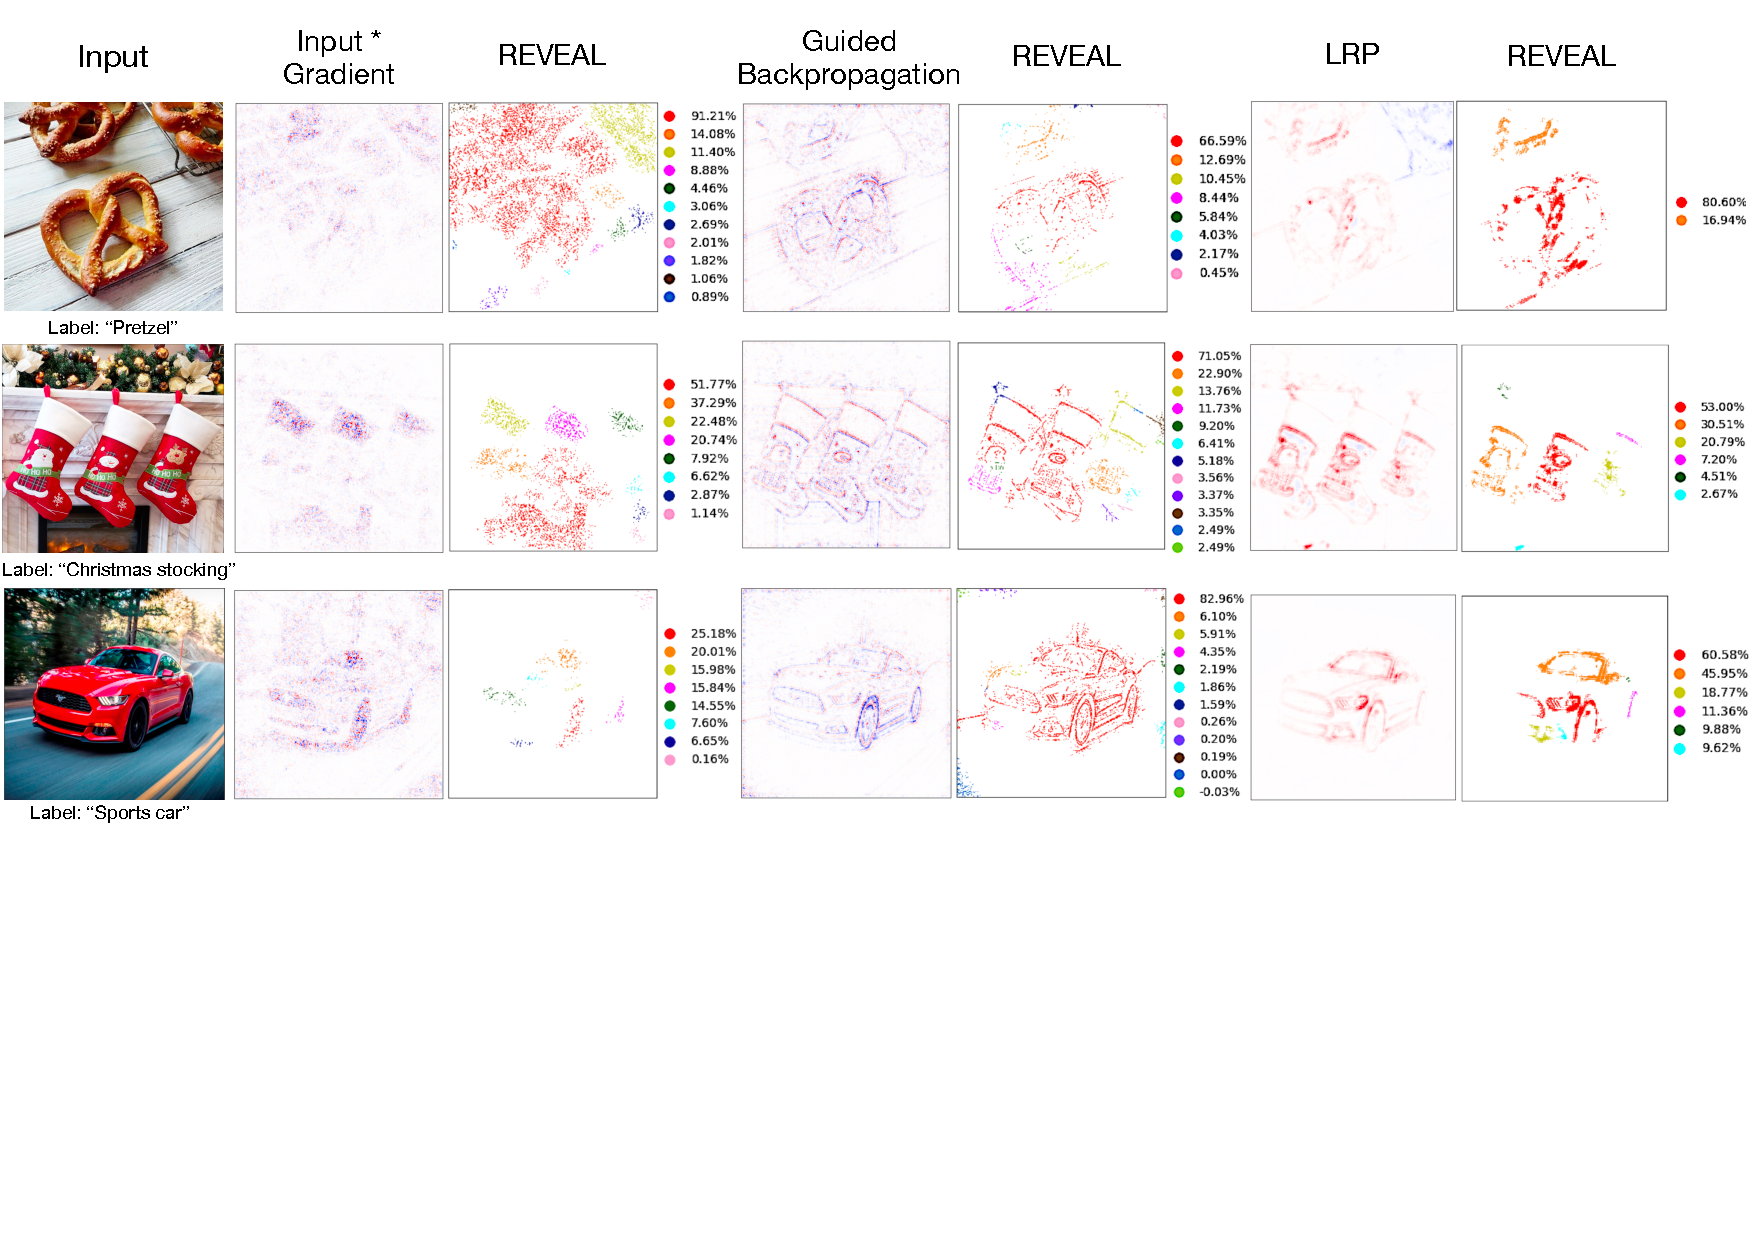
\includegraphics[width=1\linewidth]{Chapters/Results/results_section_sharp.pdf}
% 	\caption{\REVEAL\ implementation on InceptionV3. The clustering is performed to find complex features on top of heatmaps from Input$\times$Gradient, Guided BackProp, and LRP-$\alpha_1\beta_0$. }
% 	\label{fig:all}
% \end{figure*} 

% The \CTC\ value of each complex feature is then found by propagating it through the network starting from the input layer until the classification is reached. We colour all the pixels that belong to each complex feature in one colour and then use that colour in the colour-coded legend next to the heatmap to show the \CTC\ value as a percentage of the overall classification. This deviates from traditional heatmaps, where seismic colours are used to show positive relevance with the intensity of red pixels, and negative relevance with the intensity of blue.
% \begin{figure}[t!]
% \includegraphics[width=\linewidth]{Chapters/Results/contribution_vs_relevance.pdf}
% 	\caption{Examples showcasing the difference between relevance and the \CTC\ value (contribution) of a feature.}
% 	\label{fig:differnce}
% \end{figure}
% We argue that the single value of \CTC\ makes the comparison between different features easier. For example in Figure~\ref{fig:all}, when looking at \REVEAL\/'s explanation, each stocking (second row from the top) has a  \CTC\ value in isolation. One in particular (the central stocking) contributes far more than those on either side. This distinction cannot be drawn from any other technique and presents a visible difference even when each stocking is not clearly separated, as when clustering on top of \LRP\/. A similar phenomenon can be seen for the bottom plot of \ref{fig:all}, which is classified as a sports car, with the windscreen seemingly playing an equal part to the front wheel-arch and headlamp in all benchmarks when, in fact, the \CTC\ value is far greater for the wheel -- this is seen when detecting clusters on top of both Input$\times$Gradient and LRP-$\alpha_1\beta_0$.

% In Figure~\ref{fig:differnce} we show more examples that expose the difference between relevance and contribution. We have found that our technique is particularly useful when the input has features that are from two different classes that the network recognises. This brings back the point of relevance based techniques recognising edges that are relevant, but do not contribute much to the classification, as mentioned in section~\ref{subsection:contribution}. In the first example of Figure~\ref{fig:differnce} the classifier labels the input as matchsticks, \LRP\ finds both the matchsticks and the candle relevant, while putting more relevance on the candle. In contrast, \REVEAL\ shows that the matchsticks contribute more to the classification. This can also be seen in third example, where \LRP\ gives almost no relevance to the feature that contributes the most, as presented by \REVEAL\/.  

% The \CTC\ value as a percentage of the overall classification shows us how much of the classification can be explained by the feature alone. Note that the percentages don't total 100\%. As mentioned in Section~\ref{subsection:faithfulness}, this is intentional, as two distinct features may contribute to the same hidden neurons in the network and therefore have an overlapping contribution to the classification.

% As the clusters formed and evaluated by \REVEAL\ are concrete and have a single value of relevance, there is a far smaller chance of inconsistency of the interpretability. This property, as mentioned in section~\ref{subsection:contribution}, requires different users to comprehend the same information from a single explanation. While quantitative analysis is challenging as users find different explanations useful, \REVEAL\ is the only system that has predetermined and quantified complex features making it the only one that achieves that property. 

\section{Conclusion}

This chapter explored the contribution propagation rules for various types of layers commonly found in neural networks. In the upcoming chapter, we will delve into the results derived from the contribution propagation rules discussed in this chapter. By applying these rules to real-world neural network architectures, we can gain valuable insights into the behaviour and performance of these models. We will analyse the impact of each layer type on the overall network output and explore how different architectures and parameter choices affect the contribution values. Through these investigations, we aim to uncover patterns, correlations, and potential areas for improvement in neural network design and optimisation.